\section{Results}

\begin{table*}[t]
\centering
\caption{Test macro-F1 (\%) on the four financial tasks. Mean $\pm$ std over seeds where available.}
\label{tab:main}
\begin{tabular}{l r c c c c c}
\toprule
\textbf{Method} & \textbf{Params} & \textbf{FPB} & \textbf{FiQA-SA} & \textbf{TFNS} & \textbf{Headlines} & \textbf{Mean} \\
\midrule
Zero-shot & 0 & 37.3 & 51.9 & 33.5 & 45.5 & 42.0 \\
Few-shot (2/label) & 0 & 36.5 & 57.0 & 35.8 & 42.1 & 42.9 \\
Router only & 786.43K & 30.0 $\pm$ 3.5 & 21.3 $\pm$ 4.6 & 32.0 $\pm$ 2.1 & 49.6 $\pm$ 4.3 & 33.3 $\pm$ 1.3 \\
LoRA-Attn (r=16) & 2.75M & 84.2 $\pm$ 0.8 & 64.4 $\pm$ 1.6 & 82.1 $\pm$ 1.9 & 66.7 $\pm$ 14.1 & 74.3 $\pm$ 3.7 \\
LoRA-Experts (r=1) & 2.75M & 81.5 $\pm$ 1.5 & 57.6 $\pm$ 2.6 & 80.9 $\pm$ 0.1 & 43.5 $\pm$ 1.9 & 65.9 $\pm$ 1.5 \\
ESFT-Token & 128.97M & 85.7 $\pm$ 0.7 & 66.0 $\pm$ 2.7 & 84.4 $\pm$ 0.8 & 81.1 $\pm$ 1.9 & \textbf{79.3 $\pm$ 0.1} \\
ESFT-Random (ctrl) & 128.97M & 83.5 $\pm$ 0.4 & 61.3 $\pm$ 0.9 & 82.9 $\pm$ 0.6 & 73.8 $\pm$ 8.0 & 75.4 $\pm$ 2.3 \\
ESFT-Specific (ours) & 128.97M & 83.1 $\pm$ 0.9 & 59.6 $\pm$ 0.9 & 82.5 $\pm$ 0.7 & 57.9 $\pm$ 13.7 & 70.8 $\pm$ 3.3 \\
Dense Qwen2.5-0.5B LoRA-Attn & 2.16M & 84.1 $\pm$ 0.5 & 60.4 $\pm$ 0.7 & 83.5 $\pm$ 0.9 & 88.1 $\pm$ 0.9 & 79.0 $\pm$ 0.2 \\
\bottomrule
\end{tabular}
\end{table*}
\begin{table*}[t]
\centering
\caption{Test accuracy (\%).}
\label{tab:acc}
\begin{tabular}{l r c c c c c}
\toprule
\textbf{Method} & \textbf{Params} & \textbf{FPB} & \textbf{FiQA-SA} & \textbf{TFNS} & \textbf{Headlines} & \textbf{Mean} \\
\midrule
Zero-shot & 0 & 37.6 & 70.6 & 33.3 & 63.2 & 51.2 \\
Few-shot (2/label) & 0 & 35.7 & 76.6 & 34.7 & 69.5 & 54.1 \\
Router only & 786.43K & 54.6 $\pm$ 1.2 & 26.5 $\pm$ 6.7 & 47.9 $\pm$ 9.4 & 62.8 $\pm$ 2.1 & 47.9 $\pm$ 0.8 \\
LoRA-Attn (r=16) & 2.75M & 84.6 $\pm$ 0.5 & 82.0 $\pm$ 0.5 & 85.4 $\pm$ 2.5 & 76.6 $\pm$ 6.1 & 82.1 $\pm$ 2.0 \\
LoRA-Experts (r=1) & 2.75M & 82.8 $\pm$ 1.6 & 81.4 $\pm$ 3.4 & 84.4 $\pm$ 0.6 & 69.9 $\pm$ 0.5 & 79.6 $\pm$ 1.5 \\
ESFT-Token & 128.97M & 86.5 $\pm$ 0.5 & 82.1 $\pm$ 0.9 & 87.8 $\pm$ 0.4 & 85.1 $\pm$ 1.2 & 85.4 $\pm$ 0.3 \\
ESFT-Random (ctrl) & 128.97M & 84.6 $\pm$ 0.3 & 83.4 $\pm$ 0.9 & 86.4 $\pm$ 0.5 & 81.0 $\pm$ 3.7 & 83.9 $\pm$ 0.9 \\
ESFT-Specific (ours) & 128.97M & 84.5 $\pm$ 0.5 & 82.3 $\pm$ 1.2 & 86.2 $\pm$ 0.7 & 74.5 $\pm$ 4.4 & 81.9 $\pm$ 1.1 \\
Dense Qwen2.5-0.5B LoRA-Attn & 2.16M & 84.6 $\pm$ 0.6 & 79.7 $\pm$ 1.2 & 87.1 $\pm$ 1.2 & 90.3 $\pm$ 0.6 & \textbf{85.4 $\pm$ 0.5} \\
\bottomrule
\end{tabular}
\end{table*}

\subsection{Main comparison}
Table~\ref{tab:main} gives test macro-F1 for all methods. The frozen model is weak on every
financial task (42.0\% mean); two demonstrations per label change almost nothing (42.9\%),
so the gap is not a matter of understanding the output format. All methods that update
weights inside the network close most of it.

\textbf{ESFT is the best and most stable MoE adaptation.} Updating the 82 most used experts
gives 79.3\% mean macro-F1 with a standard deviation of 0.1 over seeds, the best result on
\fpb{}, \fiqa{} and \tfns{}. It matches attention LoRA on the dense Qwen2.5-0.5B (79.0\%), whose
active size is similar. The two models differ mainly on Headlines (81.1 vs.\ 88.1), where the
dense model is better, and on \fiqa{} (66.0 vs.\ 60.4), where the MoE model is better.

\textbf{Attention beats experts at a matched budget.} With the same 2.75M trainable
parameters, LoRA in the attention projections reaches 74.3\% and rank-1 LoRA in all experts
65.9\%. Expert LoRA is behind on every task and fails on Headlines (43.5\%, below zero-shot),
i.e.\ a rank-1 update spread over 768 experts is too weak for a task that needs to relate a
question to a headline. Attention LoRA solves the sentiment tasks almost as well as ESFT but
is unstable on Headlines (78.7, 70.2 and 51.1 for the three seeds).

\textbf{The router alone cannot adapt the model.} Training only the router (0.79M parameters)
decreases the mean macro-F1 to 33.3\%, below the frozen model. Its training loss barely moves
(Fig.~\ref{fig:curves}), while its routing on the test set drifts far from the pre-trained one
(Section~\ref{sec:routing}).

Test accuracy (Table~\ref{tab:acc}) gives the same ranking: 85.4\% for both
ESFT-Token and the dense model, 83.9\% for ESFT-Random and 82.1\% for attention LoRA.

\begin{figure}[t]
\centering
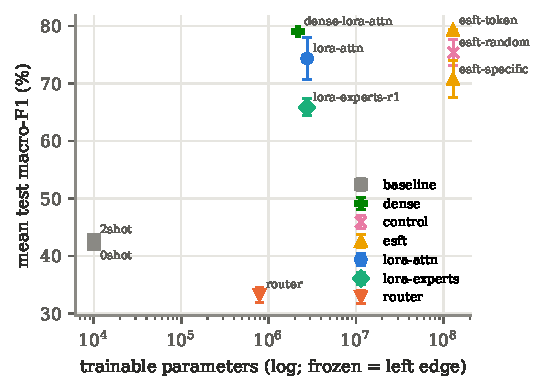
\includegraphics[width=\columnwidth]{figures/pareto}
\caption{Mean test macro-F1 against the number of trainable parameters (mean $\pm$ std over
three seeds; frozen baselines are drawn at the left edge).}
\label{fig:pareto}
\end{figure}

\subsection{Which experts to tune}
The three ESFT variants train the same number of experts in every layer and therefore exactly
the same number of parameters. The choice still matters: ESFT-Token (79.3\%) is ahead of
random experts (75.4\%), which are ahead of our domain-specific selection (70.8\%). The
difference between the variants is again largest on Headlines.

To explain the order, Table~\ref{tab:coverage} measures, for each selection, the share of all
routing decisions on the financial training data that go to the selected experts. Usage-based
selection covers 22.8\% of the routed tokens with 10.7\% of the experts. Random experts cover
roughly their share (10.7\%). The domain-specific experts are the most selective: they are
chosen 1.9 times more often on financial than on general text (9.3\% vs.\ 5.0\%), but they
see fewer financial tokens than random ones. The ranking of macro-F1 follows the coverage
exactly. A tuned expert can only change the output for the tokens routed to it, so the
amount of computation that passes through the adapted parameters, rather than their
specialisation, determines how much the model can change.

\begin{table}[t]
\centering
\caption{Share of routing decisions (top-$k$ slots, averaged over layers) that go to the
experts selected by each ESFT variant, on financial training data and on SST-2. All variants
select 82 of 768 experts (10.7\%).}
\label{tab:coverage}
\begin{tabular}{l c c c}
\toprule
Selection & Financial & General & Mean F1 \\
\midrule
ESFT-Token & 22.8 & 21.0 & 79.3 \\
ESFT-Random & 10.7 & 10.5 & 75.4 \\
ESFT-Specific & 9.3 & 5.0 & 70.8 \\
\bottomrule
\end{tabular}
\end{table}

\subsection{Routing analysis}
\label{sec:routing}

\begin{figure*}[t]
\centering
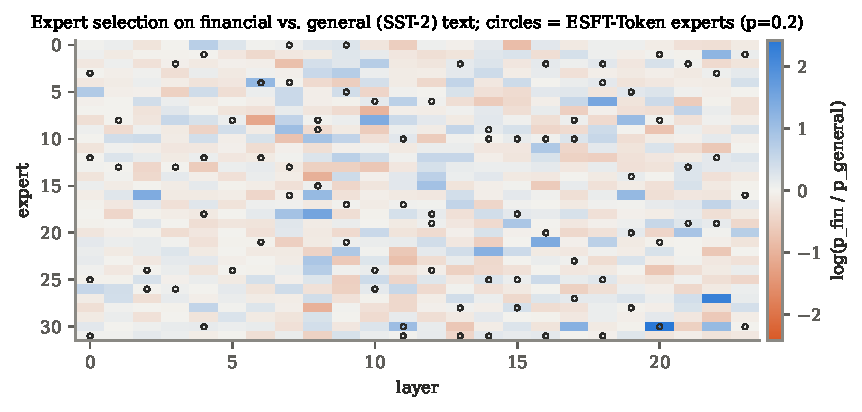
\includegraphics[width=0.85\textwidth]{figures/domain_specificity}
\caption{Domain specificity $\sigma_{\ell,e}$ of every expert of the frozen model (blue: used
more on financial text, orange: more on SST-2). Circles mark the experts selected by
ESFT-Token; most of them lie on neutral cells.}
\label{fig:spec}
\end{figure*}

\textbf{Financial text is routed differently, but only slightly.} Fig.~\ref{fig:sim} shows the
Jensen--Shannon divergence between the per-layer expert distributions of the frozen model on
the financial training sets (up to 1000 examples each) and on SST-2. The three sentiment datasets are close to each other
($2$--$5\cdot10^{-3}$) and farther from SST-2 ($12$--$16\cdot10^{-3}$); Headlines, whose prompts
contain a question, is about as far from the sentiment tasks as SST-2 is. The router entropy is high on every dataset
(3.02--3.06 nats out of a maximum of $\ln 32=3.47$), i.e.\ the model spreads tokens over many
experts and no small group of experts is reserved for finance.

\textbf{High-usage experts are generic.} Fig.~\ref{fig:spec} shows $\sigma_{\ell,e}$ for all
experts. Specificity is concentrated in a few experts per layer, and the experts that ESFT
selects are rarely among them: they are used heavily on financial and on general text alike
(Table~\ref{tab:coverage}). ESFT therefore works not because it finds ``financial experts'',
but because it adapts the experts that handle the largest part of the computation.

\textbf{Router tuning moves the routing far more than the domain does.} Fig.~\ref{fig:shift}
compares the routing of every fine-tuned model with the frozen one on the same test inputs.
Methods that leave the router frozen change it only through the hidden states
(JS $\le 4\cdot10^{-3}$ averaged over layers). The trained router moves it by
$0.14$--$0.16$, about ten times the difference between financial and general text, and the
shift grows with depth. Sending tokens to experts that were not trained to process them
destroys more than the re-routing gains, which explains why this method is below zero-shot.

\begin{figure}[t]
\centering
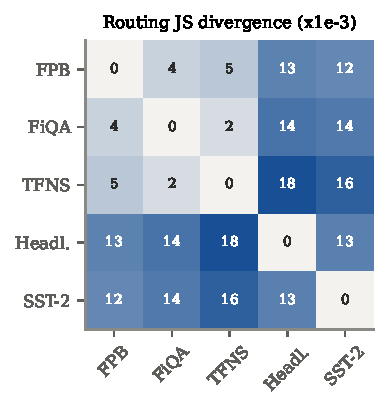
\includegraphics[width=0.78\columnwidth]{figures/task_similarity}
\caption{Routing Jensen--Shannon divergence between datasets (frozen model, financial training
data and SST-2,
averaged over layers).}
\label{fig:sim}
\end{figure}

\begin{figure}[t]
\centering
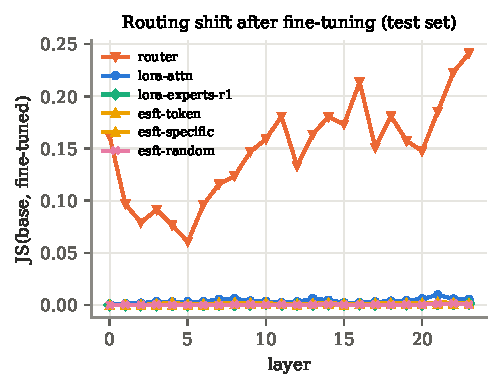
\includegraphics[width=\columnwidth]{figures/routing_shift}
\caption{Per-layer JS divergence between the routing of the frozen model and of each
fine-tuned model (seed 0) on the test sets.}
\label{fig:shift}
\end{figure}

\subsection{Error analysis}
\label{sec:errors}
Table~\ref{tab:recall} reports the recall of the classes that separate the methods, computed
from the saved test predictions and averaged over seeds.

\textbf{The frozen model ignores the neutral class.} Zero-shot, the model labels 0.1\% of the
\fpb{} sentences as neutral, although neutral is the majority class (60\% of the data); neutral
recall is 0.2\% on \fpb{} and 3.2\% on \tfns{}. This is the domain gap from the introduction in
its simplest form: factual statements such as dates, volumes and announcements are read as
positive or negative. Every method that adapts the network body raises neutral recall on
\fpb{} and \tfns{} to 86--92\%, which accounts for most of the improvement on these two tasks.
The router is the exception: it over-corrects and labels 86\% of the \fpb{} sentences as neutral.

\textbf{\fiqa{} is limited by its neutral class.} Only 8\% of the \fiqa{} training posts (about
60 examples) are neutral, and no method except the router, which over-predicts neutral
everywhere, recovers this class: neutral recall stays between 4\% and 22\%. Since macro-F1
weights the three classes equally, this caps \fiqa{} near 60--66\% for all methods, and the
ranking on this task largely follows the neutral recall (ESFT-Token is the best with 22\%).

\textbf{Headlines separates the methods through the minority class.} ``Yes'' answers are 32\%
of the Headlines data. Methods that fail on Headlines mostly stop predicting them: expert LoRA
recalls 2.5\% of them and predicts ``Yes'' for fewer than 1\% of the questions, ESFT-Specific
recalls 22\%. ESFT-Token reaches 64\% and the dense model 77\%, which explains the dense
model's lead on this task. The seed variance of attention LoRA and ESFT-Specific also comes from
this class, and it is already visible on the validation set (for attention LoRA, Headlines
validation macro-F1 is 75.7, 71.4 and 44.8 for the three seeds against 78.7, 70.2 and 51.1 on
test), so it is caused by training rather than by checkpoint selection. Questions about
headlines require relating a templated question to a short text, a different skill from
sentiment; a model that adapts few parameters, or the wrong ones, learns the majority answer.

\begin{table}[t]
\centering
\caption{Test recall (\%) of the neutral class and of ``Yes'' on Headlines, mean over seeds.}
\label{tab:recall}
\begin{tabular}{l c c c c}
\toprule
Method & \fpb{} neu. & \tfns{} neu. & \fiqa{} neu. & Headl. Yes \\
\midrule
Zero-shot & 0.2 & 3.2 & 5.6 & 10.1 \\
Router only & 85.7 & 61.6 & 57.4 & 20.8 \\
LoRA-Experts & 88.7 & 87.0 & 3.7 & 2.5 \\
ESFT-Specific & 88.9 & 89.9 & 5.6 & 21.7 \\
LoRA-Attn & 85.9 & 87.5 & 18.5 & 43.7 \\
ESFT-Random & 88.7 & 90.2 & 7.4 & 50.4 \\
ESFT-Token & 88.7 & 91.5 & 22.2 & 64.3 \\
Dense LoRA-Attn & 88.3 & 91.4 & 11.1 & 77.3 \\
\bottomrule
\end{tabular}
\end{table}

\subsection{Efficiency}
Table~\ref{tab:eff} reports the cost of one run on a T4. ESFT trains 47 times more parameters
than attention LoRA, but the stored adapter is still only 9.7\% of the model, training takes
7 minutes, and the peak memory (12.0\,GB) is 1.7\,GB above LoRA, mostly for the Adam state of
the selected experts. Expert LoRA is the most expensive method in time and memory although it
has few parameters, because every expert is touched and the adapters are applied in a Python
loop over experts. The dense model is about twice as fast and needs half the memory: at this
scale the MoE model has no efficiency advantage in our implementation.

\begin{table}[t]
\centering
\caption{Cost per run on one T4 (mean over seeds): trainable parameters, training time,
peak memory and test latency per example (batch 16).}
\label{tab:eff}
\begin{tabular}{l r r r r}
\toprule
Method & Params & Min & GB & ms \\
\midrule
Router only & 0.79M & 4.7 & 9.3 & 8.9 \\
LoRA-Attn & 2.75M & 5.0 & 10.2 & 9.5 \\
LoRA-Experts & 2.75M & 14.6 & 13.4 & 25.6 \\
ESFT (any) & 129.0M & 6.2--6.9 & 11.5--12.0 & 12.4--13.3 \\
Dense LoRA-Attn & 2.16M & 2.5 & 5.5 & 5.2 \\
\bottomrule
\end{tabular}
\end{table}

\begin{figure}[t]
\centering
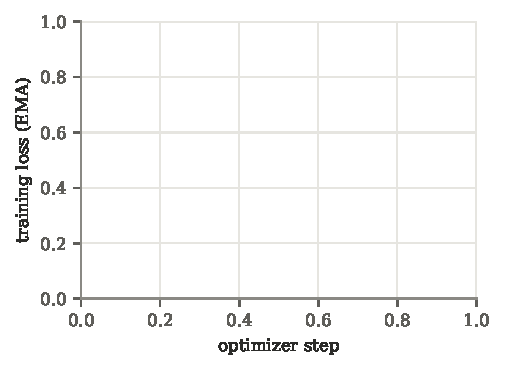
\includegraphics[width=\columnwidth]{figures/training_curves}
\caption{Training loss (exponential moving average, seed 0).}
\label{fig:curves}
\end{figure}
